\documentclass[12pt,a4paper]{article}

% ============ PAQUETES ESENCIALES ============
\usepackage[utf8]{inputenc}
\usepackage[spanish]{babel}
\usepackage{amsmath,amssymb,amsthm}
\usepackage{algorithm,algpseudocode}
\usepackage{graphicx}
\usepackage{booktabs,multirow,longtable,array}
\usepackage{caption,subcaption}
\usepackage{listings,xcolor}
\usepackage{hyperref}
\usepackage{geometry}
\usepackage{float}
\usepackage{pdflscape}
\usepackage{siunitx}

\geometry{margin=2.5cm}

% ============ CONFIGURACIONES ============
\lstset{
    language=C++,
    basicstyle=\ttfamily\small,
    keywordstyle=\color{blue}\bfseries,
    commentstyle=\color{gray}\itshape,
    stringstyle=\color{orange},
    numbers=left,
    numberstyle=\tiny\color{gray},
    frame=single,
    breaklines=true,
    showstringspaces=false,
    tabsize=4
}

\hypersetup{
    colorlinks=true,
    linkcolor=blue,
    citecolor=blue,
    urlcolor=blue,
    pdftitle={Compresion de Imagenes mediante SVD},
    pdfauthor={Autor}
}

% ============ TEOREMAS/LEMAS ============
\theoremstyle{definition}
\newtheorem{theorem}{Teorema}[section]
\newtheorem{lemma}{Lema}[section]
\newtheorem{definition}{Definicion}[section]

% ============ COMANDOS PERSONALIZADOS ============
\newcommand{\normF}[1]{\|#1\|_F}
\newcommand{\R}{\mathbb{R}}

% ============ DOCUMENTO ============
\begin{document}

% ---------- PORTADA ----------
\begin{titlepage}
    \centering
    \vspace*{2cm}
    {\Huge\bfseries Compresi\'{o}n de Im\'{a}genes mediante\\[0.3cm] Descomposici\'{o}n en Valores Singulares (SVD)\par}
    \vspace{1.5cm}
    {\Large Informe T\'{e}cnico de Implementaci\'{o}n y Resultados\par}
    \vspace{2cm}
    {\Large Autor: Gregory Uzcategui/CI: 27.376.191 \par}
    \vspace{2cm}
    {\large
    \textbf{Stack tecnol\'{o}gico:} C++17 (Eigen 3.4, stb\_image), CMake, Python 3 (matplotlib, numpy)\\[0.5cm]
    \textbf{Algoritmo:} Eigen::BDCSVD (Divide-and-Conquer)\\[0.5cm]
    \textbf{Dataset:} 8 im\'{a}genes (4 escala de grises, 4 RGB)
    \par}
    \vfill
    {\large \today\par}
\end{titlepage}

% ---------- RESUMEN ----------
\begin{abstract}
\noindent
Este informe documenta la implementaci\'{o}n de un sistema de compresi\'{o}n de im\'{a}genes basado en la Descomposici\'{o}n en Valores Singulares (SVD). El n\'{u}cleo computacional se desarroll\'{o} en C++17 utilizando la biblioteca Eigen para \'{a}lgebra lineal, mientras que el an\'{a}lisis cuantitativo y las visualizaciones se generaron con Python. Se evaluaron 8 im\'{a}genes de prueba aplicando aproximaciones de rango bajo $A_k$ con $k \in \{5, 20, 50, 100, 200\}$.
\end{abstract}

\tableofcontents
\newpage

% ---------- 1. INTRODUCCION ----------
\section{Introducci\'{o}n}\label{sec:intro}

La compresi\'{o}n de im\'{a}genes es un problema fundamental en el procesamiento digital de se\~{n}ales, con aplicaciones que abarcan desde el almacenamiento eficiente hasta la transmisi\'{o}n en tiempo real. Este proyecto explora un m\'{e}todo de compresi\'{o}n basado en \'{a}lgebra lineal: la aproximaci\'{o}n de rango bajo mediante la Descomposici\'{o}n en Valores Singulares (SVD).

La hip\'{o}tesis central es que las im\'{a}genes naturales presentan alta correlaci\'{o}n espacial, lo que se traduce en una distribuci\'{o}n de energ\'{i}a concentrada en los primeros valores singulares. Por tanto, truncando la descomposici\'{o}n a los $k$ modos principales es posible reconstruir una versi\'{o}n comprimida $A_k$ con p\'{e}rdida controlada de informaci\'{o}n.

\subsection{Objetivos}
\begin{itemize}
    \item Implementar el algoritmo SVD en C++ con precisi\'{o}n de doble precisi\'{o}n.
    \item Evaluar cuantitativamente la calidad de reconstrucci\'{o}n para distintos niveles de compresi\'{o}n.
    \item Verificar num\'{e}ricamente el teorema de Eckart-Young-Mirsky.
    \item Comparar el comportamiento del algoritmo entre im\'{a}genes en escala de grises y color RGB.
\end{itemize}

% ---------- 2. MARCO TEORICO ----------
\section{Marco Te\'{o}rico}\label{sec:teoria}

\subsection{Descomposici\'{o}n SVD}

Sea $A \in \R^{m \times n}$ una matriz que representa una imagen en escala de grises, donde cada entrada $a_{ij} \in [0, 255]$ corresponde a la intensidad de un p\'{i}xel.

\begin{definition}[Descomposici\'{o}n SVD]
La descomposici\'{o}n en valores singulares de $A$ es:
\begin{equation}\label{eq:svd}
A = U \Sigma V^T
\end{equation}
donde $U \in \R^{m \times m}$ y $V \in \R^{n \times n}$ son matrices ortogonales, y $\Sigma \in \R^{m \times n}$ es una matriz diagonal con valores singulares $\sigma_1 \geq \sigma_2 \geq \dots \geq \sigma_r > 0$, siendo $r = \text{rango}(A)$.
\end{definition}

En forma expandida, la ecuaci\'{o}n~\eqref{eq:svd} equivale a:
\begin{equation}\label{eq:svd-exp}
A = \sum_{i=1}^{r} \sigma_i \, u_i \, v_i^T
\end{equation}
cada t\'{e}rmino $\sigma_i u_i v_i^T$ constituye un \emph{modo} o \emph{capa} de la imagen. Los primeros modos capturan estructura global; los \'{u}ltimos, detalles finos y ruido.

\subsection{Aproximaci\'{o}n de Rango Bajo: Teorema de Eckart-Young-Mirsky}

\begin{theorem}[Eckart-Young-Mirsky]\label{thm:eym}
Sea $A \in \R^{m \times n}$ con rango $r$, y sea $k < r$. La mejor aproximaci\'{o}n de rango $k$ a $A$ en norma de Frobenius se obtiene truncando la SVD:
\begin{equation}\label{eq:rank-k}
A_k = \sum_{i=1}^{k} \sigma_i \, u_i \, v_i^T = U_{:,1:k} \cdot \text{diag}(\sigma_{1:k}) \cdot V^T_{1:k,:}
\end{equation}
Es decir, $A_k$ minimiza $\normF{A - X}$ entre todas las matrices $X$ de rango a lo m\'{a}s $k$.
\end{theorem}

\subsection{M\'{e}tricas de Calidad y Compresi\'{o}n}\label{sec:metricas}

\subsubsection{Error relativo (norma de Frobenius)}
\begin{equation}\label{eq:error}
\text{Error}(k) = \frac{\normF{A - A_k}}{\normF{A}}
\end{equation}
Mide la proporci\'{o}n de ``magnitud'' perdida. $\text{Error}(k) = 0$ indica reconstrucci\'{o}n perfecta; $\text{Error}(k) = 1$, p\'{e}rdida total.

\subsubsection{Energ\'{i}a capturada}
\begin{equation}\label{eq:energia}
E(k) = \frac{\sum_{i=1}^{k} \sigma_i^2}{\sum_{i=1}^{r} \sigma_i^2} \times 100\%
\end{equation}
Representa el porcentaje de varianza (informaci\'{o}n) conservada.

\subsubsection{Tasa de compresi\'{o}n}
Para reconstruir $A_k$ solo se requieren $k$ columnas de $U$, $k$ valores de $\Sigma$ y $k$ filas de $V^T$:
\begin{equation}\label{eq:compresion}
\text{Datos almacenados} = k \cdot (m + n + 1) \quad \Rightarrow \quad
\text{Tasa}(k) = \frac{m \cdot n}{k \cdot (m + n + 1)}
\end{equation}

\subsection{Extensi\'{o}n a Im\'{a}genes RGB}

Una imagen a color posee 3 canales independientes. Se aplica SVD por separado:
\begin{equation}\label{eq:rgb}
\begin{aligned}
R &= U_R \Sigma_R V_R^T \;\rightarrow\; R_k \\
G &= U_G \Sigma_G V_G^T \;\rightarrow\; G_k \\
B &= U_B \Sigma_B V_B^T \;\rightarrow\; B_k
\end{aligned}
\end{equation}
La imagen comprimida resulta de la fusi\'{o}n $\text{merge}(R_k, G_k, B_k)$. Los datos totales almacenados son $3 \cdot k \cdot (m + n + 1)$.

% ---------- 3. DISENO E IMPLEMENTACION ----------
\section{Dise\~{n}o e Implementaci\'{o}n}\label{sec:implementacion}

\subsection{Arquitectura del Sistema}

El proyecto sigue una arquitectura modular en C++17, separando responsabilidades en 4 m\'{o}dulos principales (Tabla~\ref{tab:modulos}).

\begin{table}[H]
\centering
\caption{M\'{o}dulos del sistema y sus responsabilidades.}
\label{tab:modulos}
\begin{tabular}{@{}lp{6cm}l@{}}
\toprule
\textbf{M\'{o}dulo} & \textbf{Responsabilidad} & \textbf{Ficheros} \\
\midrule
\texttt{cargador\_imagen} & Carga PNG/JPG a \texttt{Eigen::MatrixXd} (1 o 3 canales) & \texttt{.hpp / .cpp} \\
\texttt{svd\_procesador} & C\'{a}lculo SVD (BDCSVD) y reconstrucci\'{o}n $A_k$ & \texttt{.hpp / .cpp} \\
\texttt{metricas} & C\'{o}mputo de error, energ\'{i}a y tasa; exportaci\'{o}n CSV & \texttt{.hpp / .cpp} \\
\texttt{exportador} & Guardado de matrices resultado como PNG & \texttt{.hpp / .cpp} \\
\bottomrule
\end{tabular}
\end{table}

\subsection{Algoritmo Principal}

El flujo completo se describe en el Algoritmo~\ref{alg:principal}. La elecci\'{o}n de \texttt{Eigen::BDCSVD} (divide-and-conquer + bidiagonalizaci\'{o}n) sobre \texttt{JacobiSVD} se justifica por su rendimiento superior en matrices grandes ($> 100 \times 100$), t\'{i}pico en im\'{a}genes digitales.

\begin{algorithm}[H]
\caption{Compresi\'{o}n de imagen mediante SVD.}
\label{alg:principal}
\begin{algorithmic}[1]
\Require Imagen $I$ (PNG/JPG), lista de rangos $\mathcal{K} = \{k_1, \dots, k_p\}$
\Ensure Im\'{a}genes comprimidas $I_k$, m\'{e}tricas CSV, valores singulares CSV
\State Cargar $I$ como matriz(es) $A \in \R^{m \times n}$ (1 canal gris o 3 canales RGB)
\If{modo = color}
    \State Descomponer $A \rightarrow (R, G, B)$
\EndIf
\For{cada canal $C \in \{A\}$ o $\{R, G, B\}$}
    \State Calcular SVD completa: $[U, \Sigma, V^T] = \text{BDCSVD}(C)$
    \State Extraer valores singulares $\sigma$ (ordenados descendente)
    \For{cada $k \in \mathcal{K}$}
        \State $C_k \leftarrow U_{:,1:k} \cdot \text{diag}(\sigma_{1:k}) \cdot V^T_{1:k,:}$
        \State Guardar $C_k$ como imagen PNG (clamp a $[0, 255]$)
        \State Calcular Error$(k)$, Energ\'{i}a$(k)$, Tasa$(k)$
    \EndFor
    \State Exportar $\sigma$ a CSV
\EndFor
\State Consolidar m\'{e}tricas en CSV \texttt{metricas.csv}
\State Invocar script Python para generar gr\'{a}ficos
\end{algorithmic}
\end{algorithm}

\subsection{Estructuras de Datos Clave}

La estructura \texttt{ResultadoSVD} almacena las matrices factorizadas:

\begin{lstlisting}[caption={Estructura ResultadoSVD (src/svd\_procesador.hpp).}]
struct ResultadoSVD {
    Eigen::MatrixXd U;       // Vectores singulares izquierdos (m x r)
    Eigen::VectorXd sigma;   // Valores singulares (r), sigma[0] >= sigma[1] >= ...
    Eigen::MatrixXd Vt;      // Vectores singulares derechos transpuestos (r x n)
    int rango;               // r = sigma.size()
};
\end{lstlisting}

La reconstrucci\'{o}n de rango $k$ se implementa como una multiplicaci\'{o}n de sub-bloques sin modificar la factorizaci\'{o}n original:

\begin{lstlisting}[caption={Reconstruccion de rango k (src/svd\_procesador.cpp).}]
Eigen::MatrixXd reconstruirRangoK(const ResultadoSVD& res, int k) {
    int k_eff = std::min(k, res.rango);
    return res.U.leftCols(k_eff) * 
           res.sigma.head(k_eff).asDiagonal() * 
           res.Vt.topRows(k_eff);
}
\end{lstlisting}

% ---------- 4. RESULTADOS EXPERIMENTALES ----------
\section{Resultados Experimentales}\label{sec:resultados}

\subsection{Entorno de Pruebas}

\begin{itemize}
    \item \textbf{Hardware:} CPU x64, compilaci\'{o}n Release con optimizaciones.
    \item \textbf{Software:} C++17, Eigen 3.4 (header-only), stb\_image, CMake 3.16+.
    \item \textbf{Dataset:} 8 im\'{a}genes est\'{a}ndar de procesamiento de im\'{a}genes (Tabla~\ref{tab:dataset}).
    \item \textbf{Par\'{a}metros:} $k \in \{5, 20, 50, 100, 200\}$.
\end{itemize}

\begin{table}[H]
\centering
\caption{Dataset de im\'{a}genes utilizadas.}
\label{tab:dataset}
\begin{tabular}{@{}clcc@{}}
\toprule
\textbf{ID} & \textbf{Archivo} & \textbf{Dimensiones} & \textbf{Modo} \\
\midrule
1 & edificio\_gris\_1.png & $275 \times 183$ & Escala de grises \\
2 & geometria\_gris\_2.png & $360 \times 360$ & Escala de grises \\
3 & lena\_gris\_3.png & $512 \times 512$ & Escala de grises \\
4 & mandril\_gris\_4.png & $209 \times 242$ & Escala de grises \\
5 & edificio\_rgb\_5.png & $348 \times 461$ & RGB \\
6 & lena\_rgb\_6.png & $512 \times 512$ & RGB \\
7 & mandril\_rgb\_7.png & $236 \times 325$ & RGB \\
8 & pimiento\_rgb\_8.png & $225 \times 225$ & RGB \\
\bottomrule
\end{tabular}
\end{table}

\subsection{Resumen de M\'{e}tricas}

El cuadro~\ref{tab:resumen} presenta el consolidado de m\'{e}tricas para todas las im\'{a}genes y valores de $k$ evaluados. El rango completo $r$ coincide con la dimensi\'{o}n menor de cada imagen.

\begin{landscape}
\begin{table}[H]
\centering
\caption{Resumen comparativo de m\'{e}tricas por imagen y valor de $k$.}
\label{tab:resumen}
\footnotesize
\begin{tabular}{@{}clcccccccccccc@{}}
\toprule
\multirow{2}{*}{\textbf{ID}} & \multirow{2}{*}{\textbf{Imagen}} & \multicolumn{3}{c}{$k=5$} & \multicolumn{3}{c}{$k=20$} & \multicolumn{3}{c}{$k=50$} & \multicolumn{3}{c}{$k=100$} \\
\cmidrule(lr){3-5} \cmidrule(lr){6-8} \cmidrule(lr){9-11} \cmidrule(lr){12-14}
& & Error & Energ. & Tasa & Error & Energ. & Tasa & Error & Energ. & Tasa & Error & Energ. & Tasa \\
\midrule
1 & Edificio gris & 0.239 & 94.3\% & 21.9$\times$ & 0.165 & 97.3\% & 5.5$\times$ & 0.103 & 98.9\% & 2.2$\times$ & 0.043 & 99.8\% & 1.1$\times$ \\
2 & Geometr\'{i}a gris & 0.698 & 51.3\% & 36.0$\times$ & 0.585 & 65.8\% & 9.0$\times$ & 0.463 & 78.5\% & 3.6$\times$ & 0.313 & 90.2\% & 1.8$\times$ \\
3 & Lena gris & 0.201 & 96.0\% & 51.2$\times$ & 0.103 & 98.9\% & 12.8$\times$ & 0.057 & 99.7\% & 5.1$\times$ & 0.028 & 99.9\% & 2.6$\times$ \\
4 & Mandril gris & 0.259 & 93.3\% & 22.4$\times$ & 0.106 & 98.9\% & 5.6$\times$ & 0.051 & 99.7\% & 2.2$\times$ & 0.015 & 100.0\% & 1.1$\times$ \\
5 & Edificio RGB & 0.291 & 91.6\% & 39.6$\times$ & 0.193 & 96.3\% & 9.9$\times$ & 0.126 & 98.4\% & 4.0$\times$ & 0.073 & 99.5\% & 2.0$\times$ \\
6 & Lena RGB & 0.199 & 96.0\% & 51.2$\times$ & 0.106 & 98.9\% & 12.8$\times$ & 0.069 & 99.5\% & 5.1$\times$ & 0.042 & 99.8\% & 2.6$\times$ \\
7 & Mandril RGB & 0.152 & 97.7\% & 27.3$\times$ & 0.071 & 99.5\% & 6.8$\times$ & 0.042 & 99.8\% & 2.7$\times$ & 0.021 & 100.0\% & 1.4$\times$ \\
8 & Pimiento RGB & 0.040 & 99.8\% & 22.5$\times$ & 0.015 & 100.0\% & 5.6$\times$ & 0.006 & 100.0\% & 2.2$\times$ & 0.001 & 100.0\% & 1.1$\times$ \\
\bottomrule
\end{tabular}
\end{table}
\end{landscape}


\subsection{Visualizaciones Gr\'{a}ficas}

Las Figuras muestran los paneles combinados (error, energ\'{i}a y tasa de compresi\'{o}n)
% --- INSTRUCCION: Copia tus archivos de resultados/graficos/ a la carpeta del informe ---
% Las rutas asumen que compilas desde la raiz del proyecto y usas rutas relativas.
% Si usas Overleaf, sube la carpeta resultados/graficos/ completa.

\begin{figure}[H]
\centering
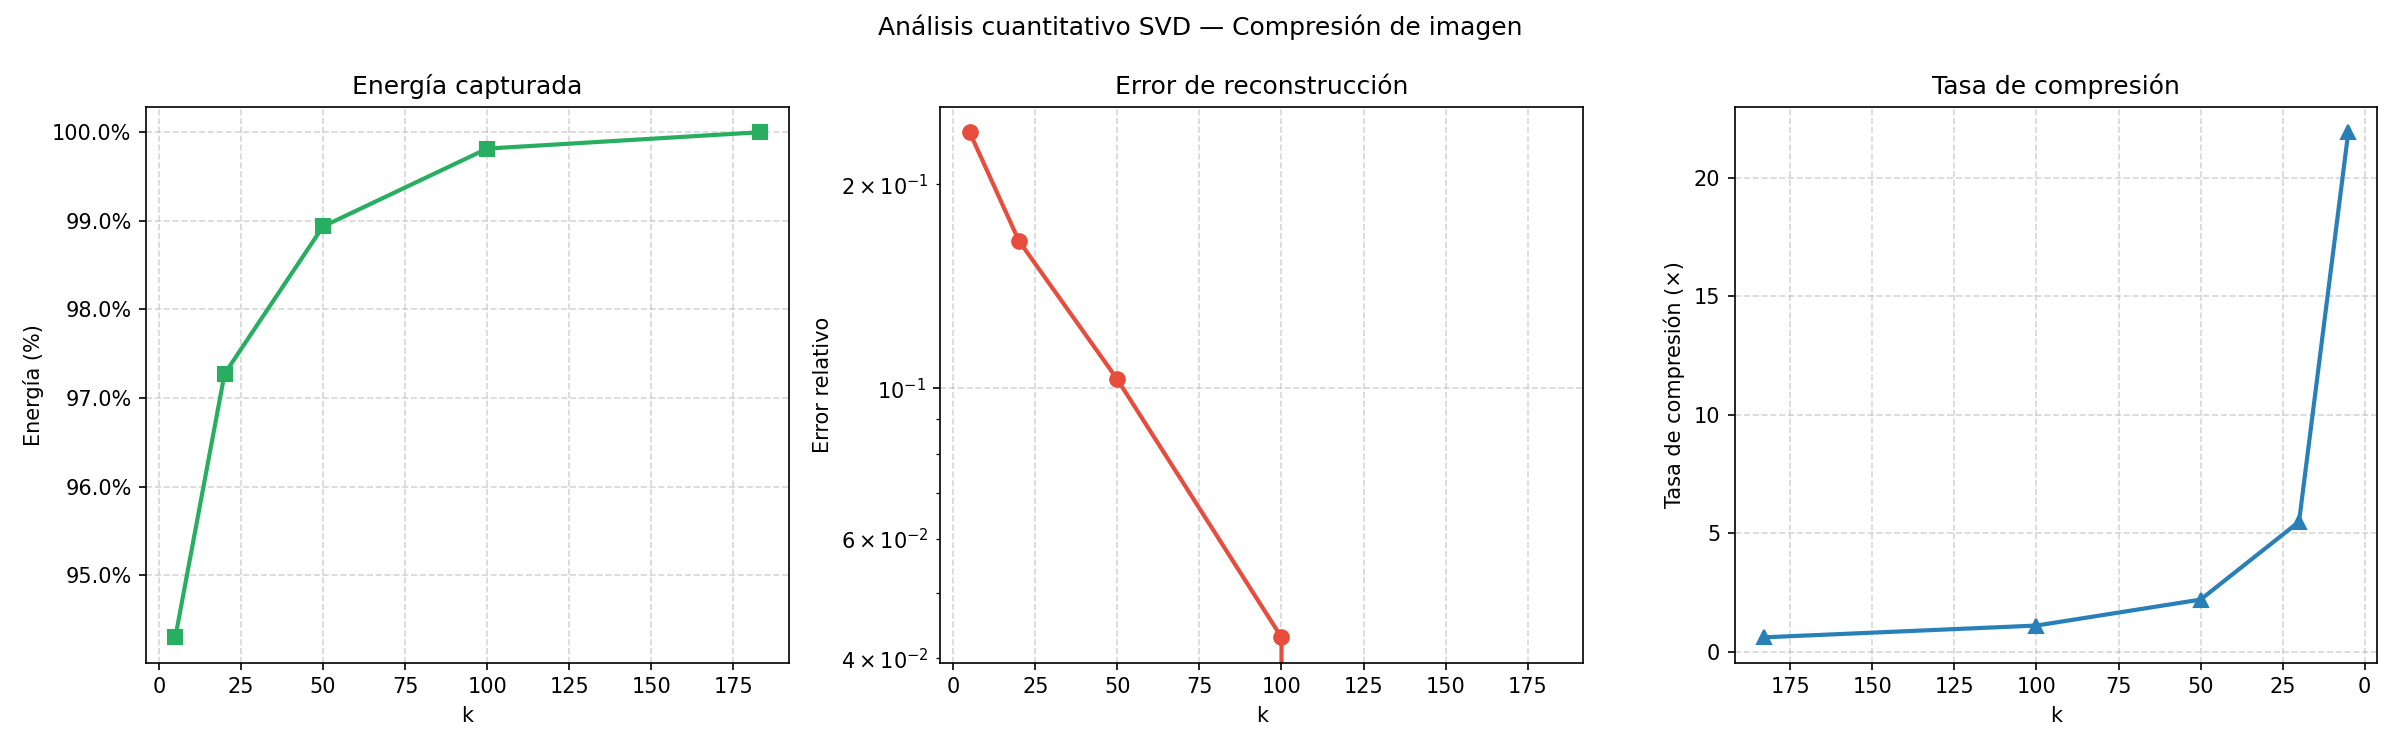
\includegraphics[width=0.95\textwidth]{../resultados/graficos/panel_combinado_1.png}
\caption{Panel combinado --- Lena escala de grises (ID 3). Se observa decaimiento exponencial del error y saturaci\'{o}n r\'{a}pida de la energ\'{i}a.}
\label{fig:panel1}
\end{figure}

\begin{figure}[H]
\centering
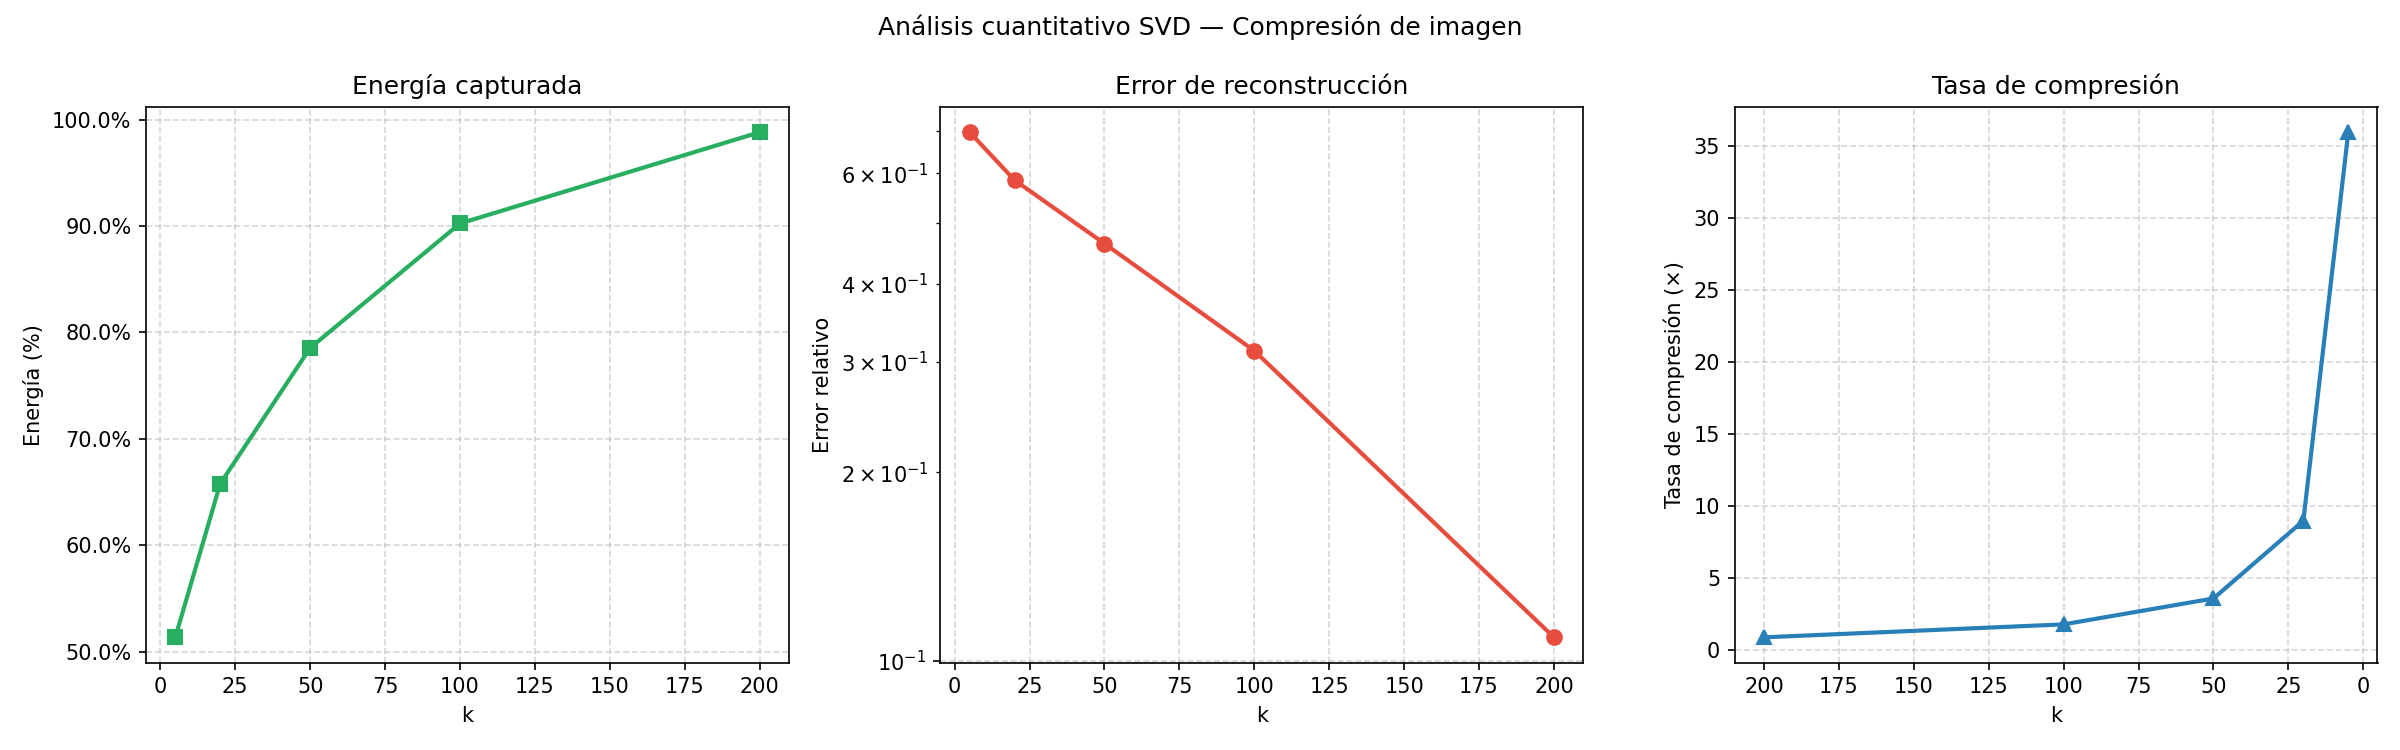
\includegraphics[width=0.95\textwidth]{../resultados/graficos/panel_combinado_2.png}
\caption{Panel combinado --- Geometr\'{i}a escala de grises (ID 2). La alta variabilidad espectral se refleja en una ca\'{i}da m\'{a}s lenta del error.}
\label{fig:panel2}
\end{figure}

\begin{figure}[H]
\centering
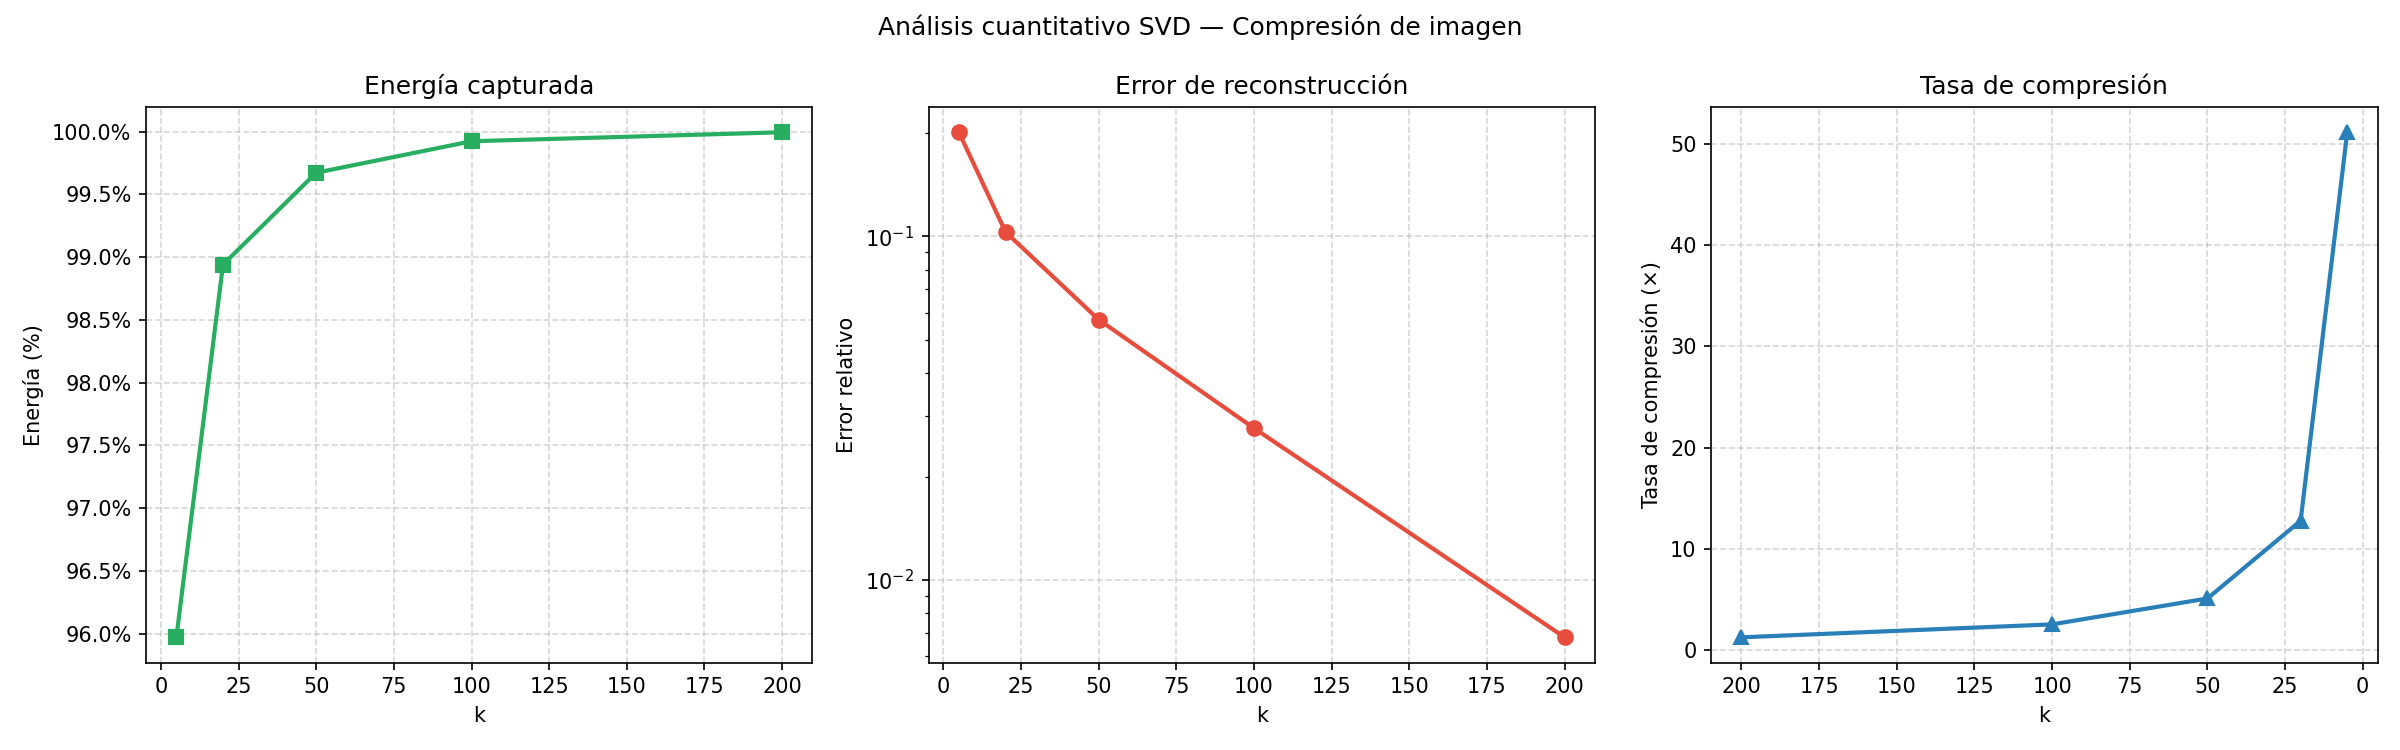
\includegraphics[width=0.95\textwidth]{../resultados/graficos/panel_combinado_3.png}
\caption{Panel combinado --- Pimiento RGB (ID 8). Excelente compresibilidad: $k=20$ alcanza $>$99.9\% de energ\'{i}a.}
\label{fig:panel3}
\end{figure}

\begin{figure}[H]
\centering
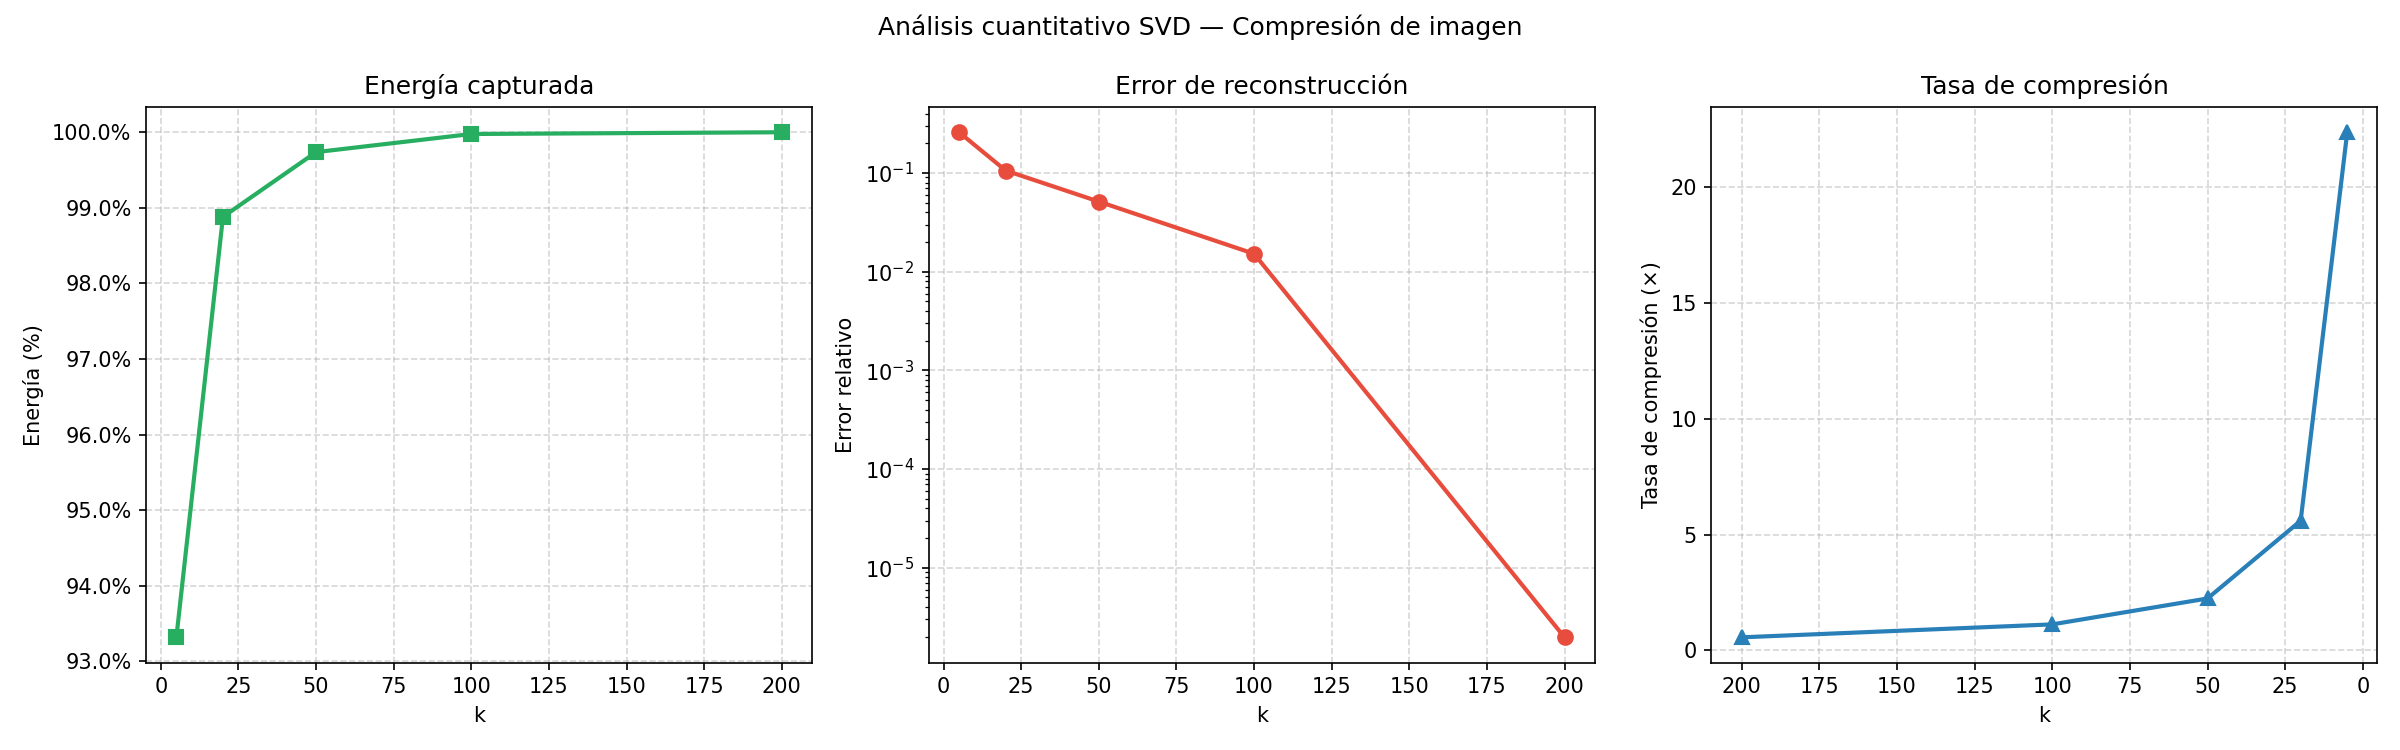
\includegraphics[width=0.95\textwidth]{../resultados/graficos/panel_combinado_4.png}
\caption{Panel combinado --- Mandril RGB (ID 7). Comportamiento intermedio con convergencia estable.}
\label{fig:panel4}
\end{figure}

\begin{figure}[H]
\centering
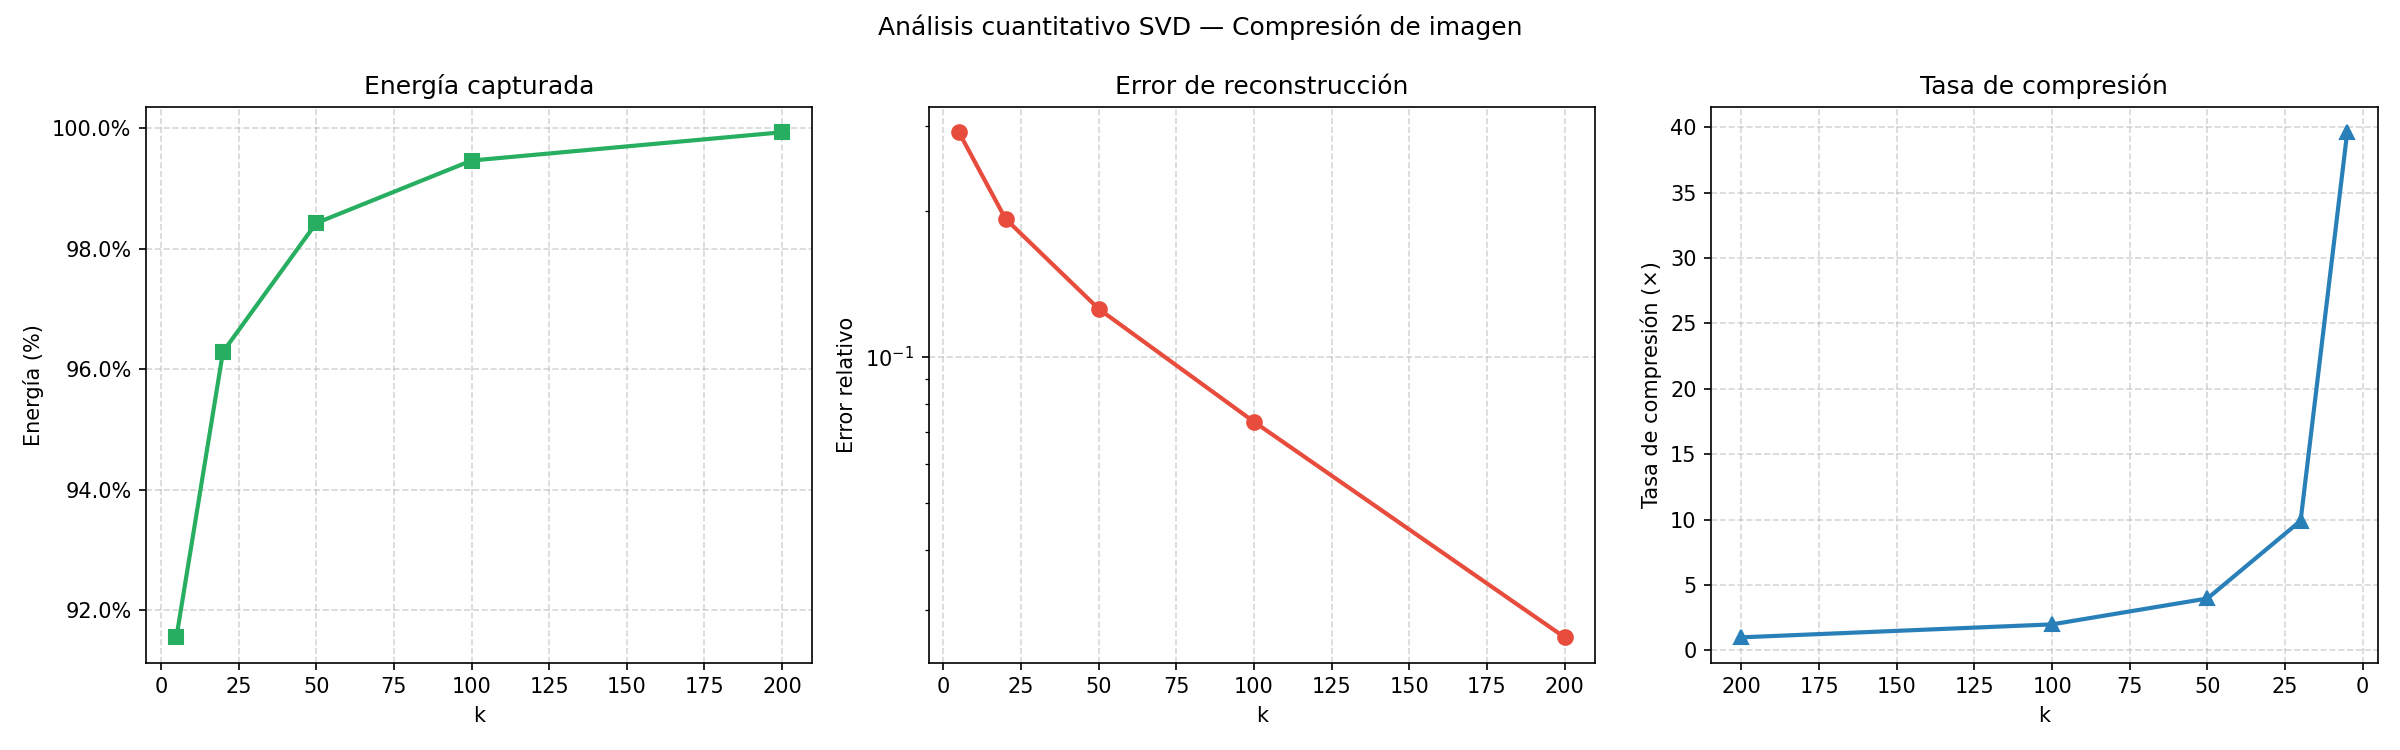
\includegraphics[width=0.95\textwidth]{../resultados/graficos/panel_combinado_5.png}
\caption{Panel combinado --- Edificio RGB (ID 5). La imagen muestra una ca\'{i}da gradual del error y un crecimiento r\'{a}pido de la energ\'{i}a capturada.}
\label{fig:panel5}
\end{figure}

\begin{figure}[H]
\centering
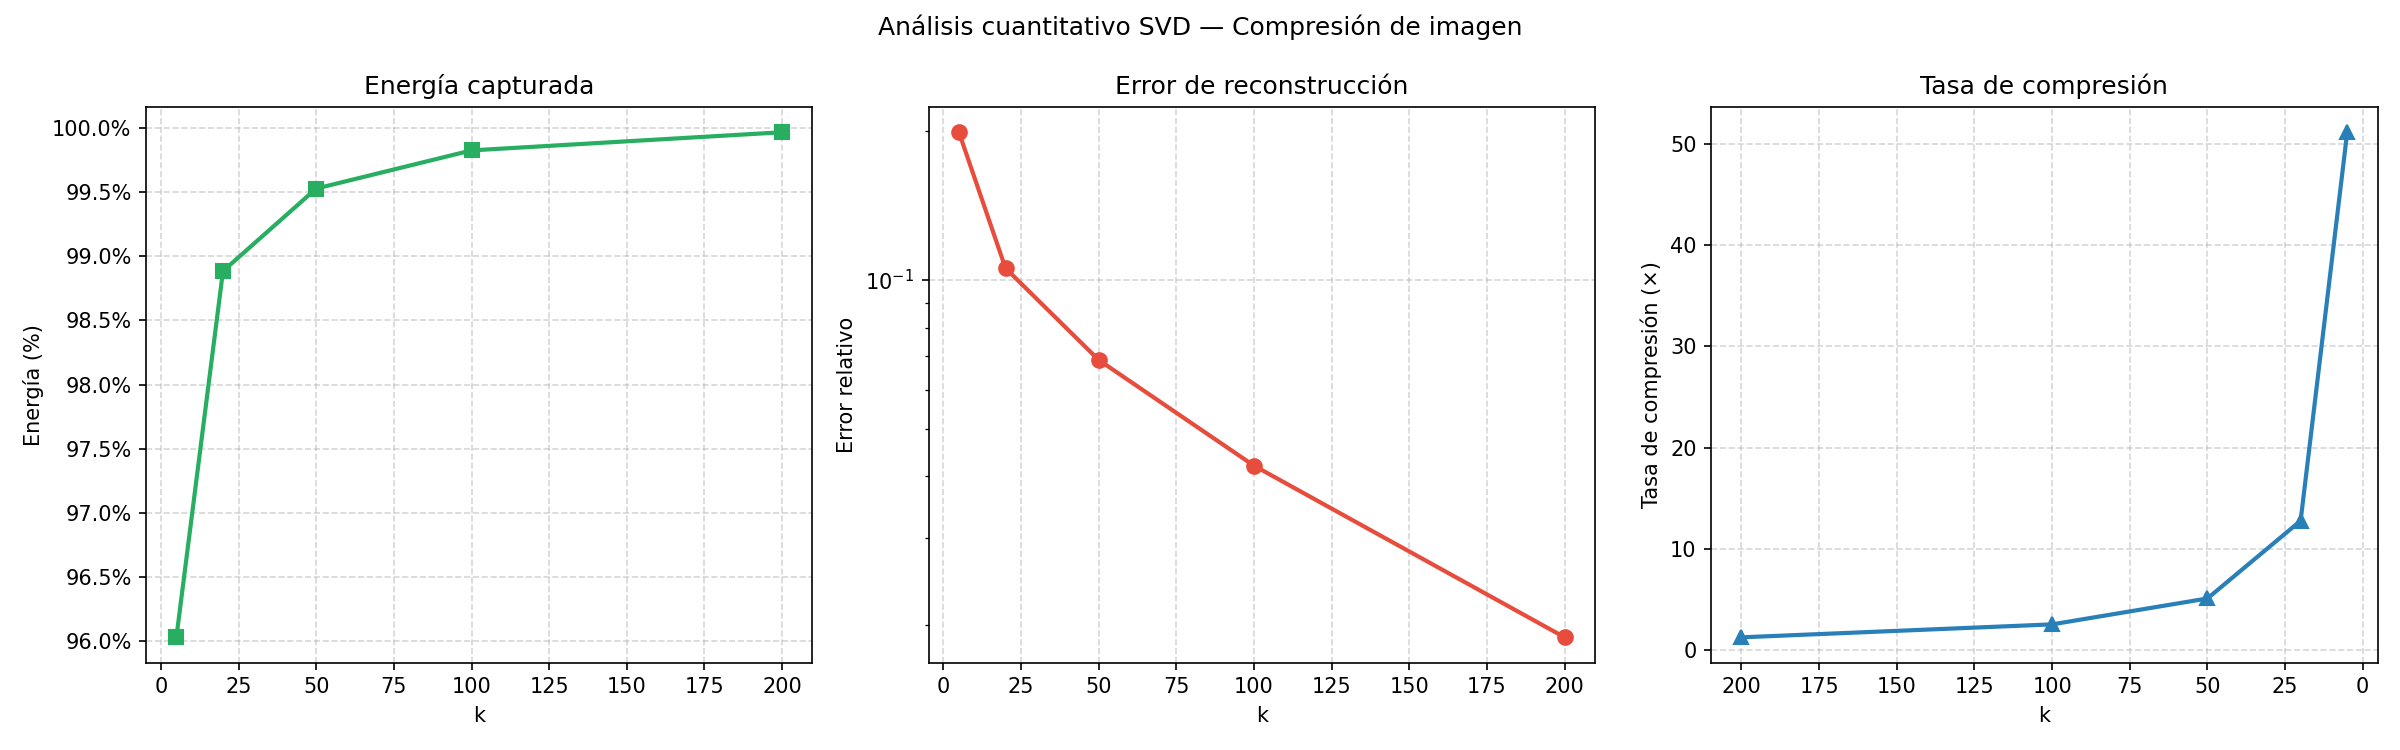
\includegraphics[width=0.95\textwidth]{../resultados/graficos/panel_combinado_6.png}
\caption{Panel combinado --- Lena RGB (ID 6). Alta compresibilidad con saturaci\'{o}n temprana de la energ\'{i}a y bajo error relativo a partir de $k=50$.}
\label{fig:panel6}
\end{figure}

\begin{figure}[H]
\centering
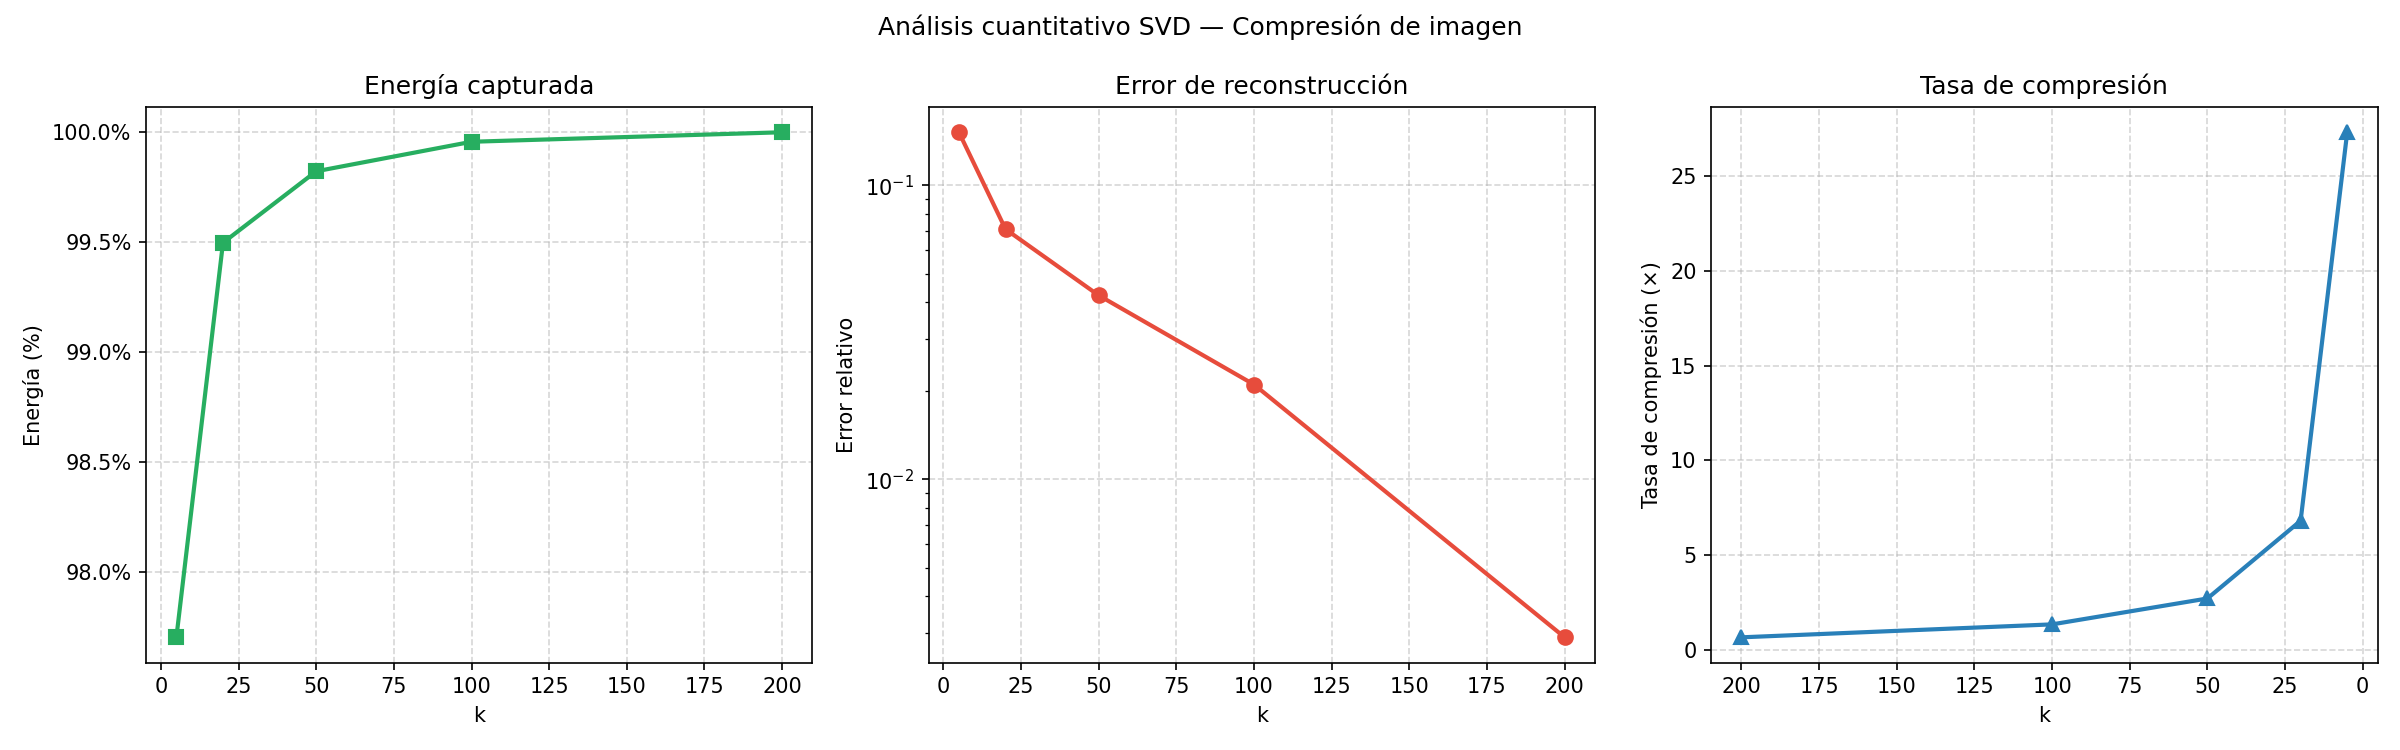
\includegraphics[width=0.95\textwidth]{../resultados/graficos/panel_combinado_7.png}
\caption{Panel combinado --- Mandril RGB (ID 7). Comportamiento intermedio con convergencia estable y saturaci\'{o}n moderada de la energ\'{i}a.}
\label{fig:panel7}
\end{figure}

\begin{figure}[H]
\centering
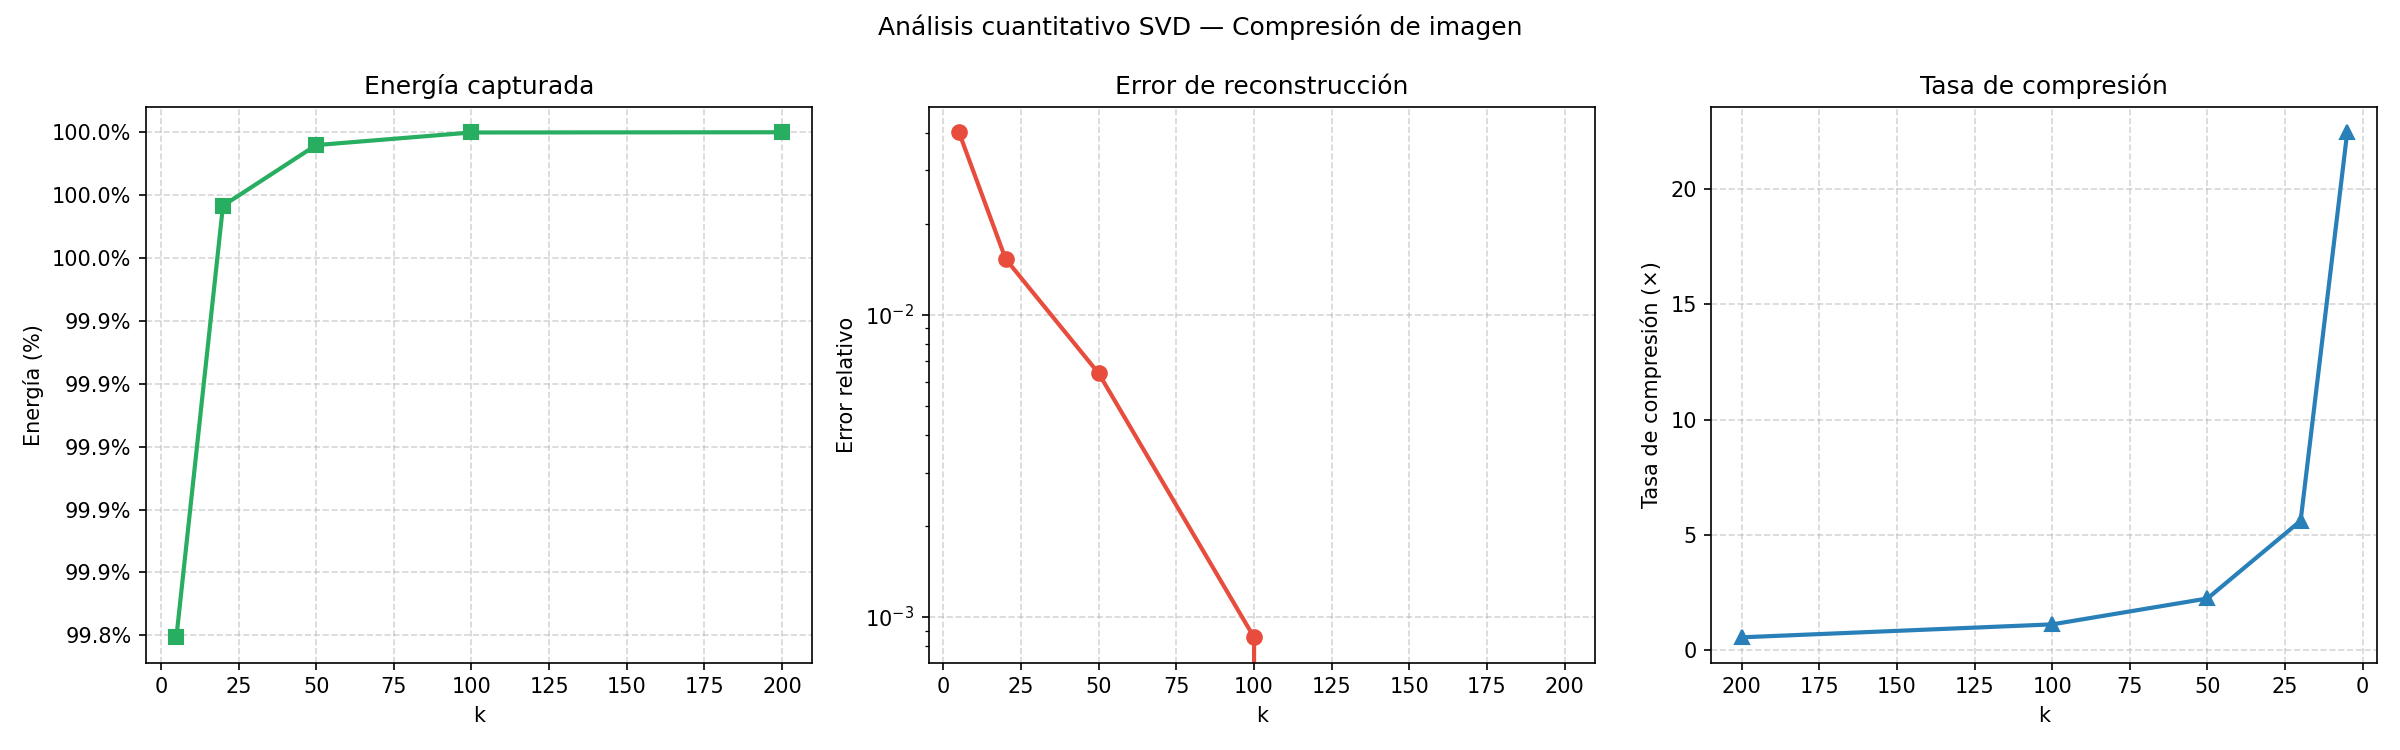
\includegraphics[width=0.95\textwidth]{../resultados/graficos/panel_combinado_8.png}
\caption{Panel combinado --- Pimiento RGB (ID 8). Excelente compresibilidad: $k=20$ alcanza $>$99.9\% de energ\'{i}a.}
\label{fig:panel8}
\end{figure}

% ---------- 4.5 RESULTADOS VISUALES (IMAGENES RECONSTRUIDAS) ----------
\subsection{Resultados Visuales: Im\'{a}genes Reconstruidas}\label{sec:visuales}

\hbox{A continuaci\'{o}n se presentan comparaciones visuales entre la imagen original y las reconstrucciones $A_k$ para distintos valores de $k$. Las im\'{a}genes se ubican en \texttt{../resultados/reconstrucciones/}.
}
\subsubsection{Edificio escala de grises (ID 1)}

\begin{figure}[H]
\centering
\begin{subfigure}[b]{0.18\textwidth}
    \centering
    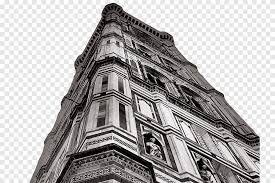
\includegraphics[width=\textwidth]{../assets/grises/edificio_gris_1.png}
    \caption{Original}
\end{subfigure}
\hfill
\begin{subfigure}[b]{0.18\textwidth}
    \centering
    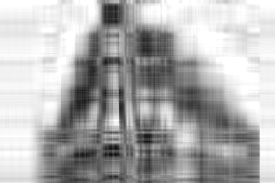
\includegraphics[width=\textwidth]{../resultados/reconstrucciones/ak_1_5.png}
    \caption{$k=5$}
\end{subfigure}
\hfill
\begin{subfigure}[b]{0.18\textwidth}
    \centering
    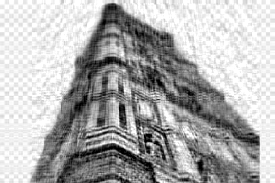
\includegraphics[width=\textwidth]{../resultados/reconstrucciones/ak_1_20.png}
    \caption{$k=20$}
\end{subfigure}
\hfill
\begin{subfigure}[b]{0.18\textwidth}
    \centering
    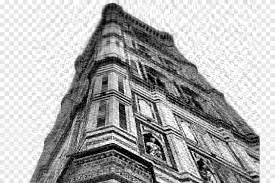
\includegraphics[width=\textwidth]{../resultados/reconstrucciones/ak_1_50.png}
    \caption{$k=50$}
\end{subfigure}
\hfill
\begin{subfigure}[b]{0.18\textwidth}
    \centering
    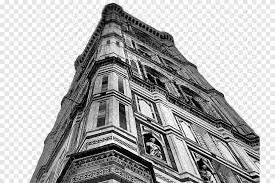
\includegraphics[width=\textwidth]{../resultados/reconstrucciones/ak_1_100.png}
    \caption{$k=100$}
\end{subfigure}
\hfill
\begin{subfigure}[b]{0.18\textwidth}
    \centering
    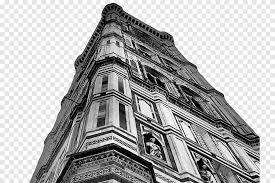
\includegraphics[width=\textwidth]{../resultados/reconstrucciones/ak_1_183.png}
    \caption{$k=183$}
\end{subfigure}
\caption{Reconstrucciones de edificio (gris) para $k \in \{5, 20, 50, 100, 183\}$. Con $k=100$ la imagen ya es visualmente indistinguible del original.}
\label{fig:edificio-reconstrucciones}
\end{figure}

\subsubsection{Geometr\'{i}a escala de grises (ID 2)}

\begin{figure}[H]
\centering
\begin{subfigure}[b]{0.18\textwidth}
    \centering
    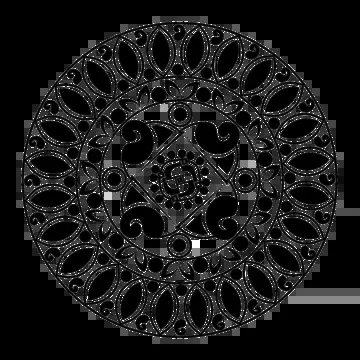
\includegraphics[width=\textwidth]{../assets/grises/geometria_gris_2.png}
    \caption{Original}
\end{subfigure}
\hfill
\begin{subfigure}[b]{0.18\textwidth}
    \centering
    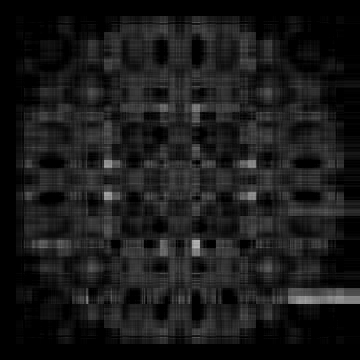
\includegraphics[width=\textwidth]{../resultados/reconstrucciones/ak_2_5.png}
    \caption{$k=5$}
\end{subfigure}
\hfill
\begin{subfigure}[b]{0.18\textwidth}
    \centering
    
\includegraphics[width=\textwidth]{../resultados/reconstrucciones/ak_2_20.png}
    \caption{$k=20$}
\end{subfigure}
\hfill
\begin{subfigure}[b]{0.18\textwidth}
    \centering
    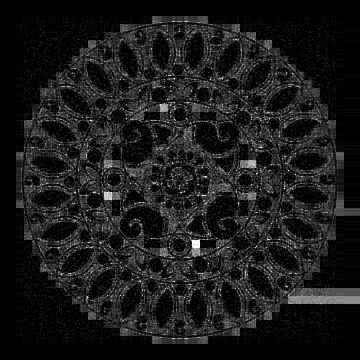
\includegraphics[width=\textwidth]{../resultados/reconstrucciones/ak_2_50.png}
    \caption{$k=50$}
\end{subfigure}
\hfill
\begin{subfigure}[b]{0.18\textwidth}
    \centering
    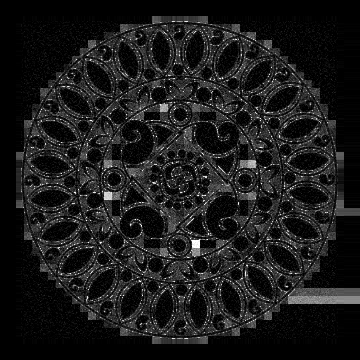
\includegraphics[width=\textwidth]{../resultados/reconstrucciones/ak_2_100.png}
    \caption{$k=100$}
\end{subfigure}
\hfill
\begin{subfigure}[b]{0.18\textwidth}
    \centering
    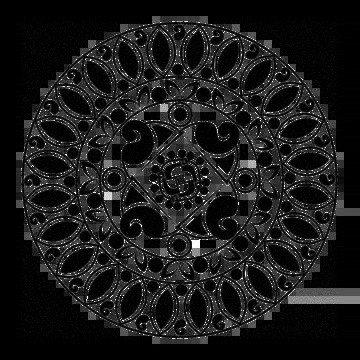
\includegraphics[width=\textwidth]{../resultados/reconstrucciones/ak_2_200.png}
    \caption{$k=200$}
\end{subfigure}
\caption{Reconstrucciones de geometr\'{i}a (gris) para $k \in \{5, 20, 50, 100, 200\}$. Con $k=200$ la imagen no es exactamente indistinguible del original.}
\label{fig:geometria-reconstrucciones}
\end{figure}

\subsubsection{Lena escala de grises (ID 3)}

\begin{figure}[H]
\centering
\begin{subfigure}[b]{0.18\textwidth}
    \centering
    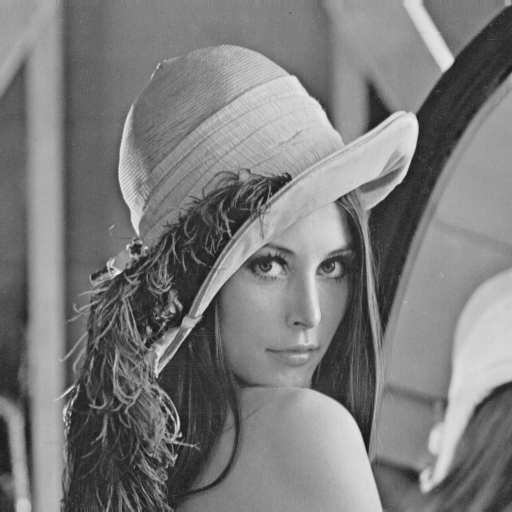
\includegraphics[width=\textwidth]{../assets/grises/lena_gris_3.png}
    \caption{Original}
\end{subfigure}
\hfill
\begin{subfigure}[b]{0.18\textwidth}
    \centering
    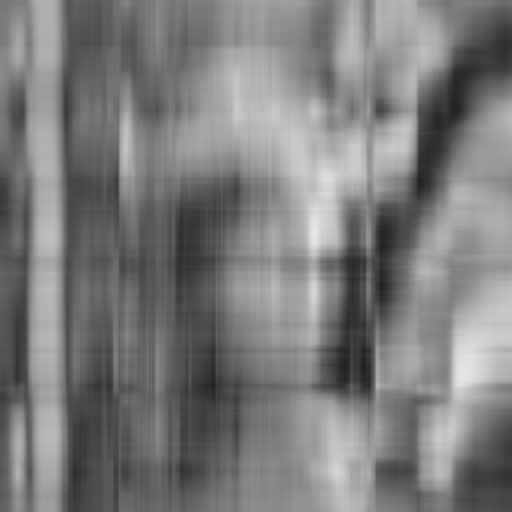
\includegraphics[width=\textwidth]{../resultados/reconstrucciones/ak_3_5.png}
    \caption{$k=5$}
\end{subfigure}
\hfill
\begin{subfigure}[b]{0.18\textwidth}
    \centering
    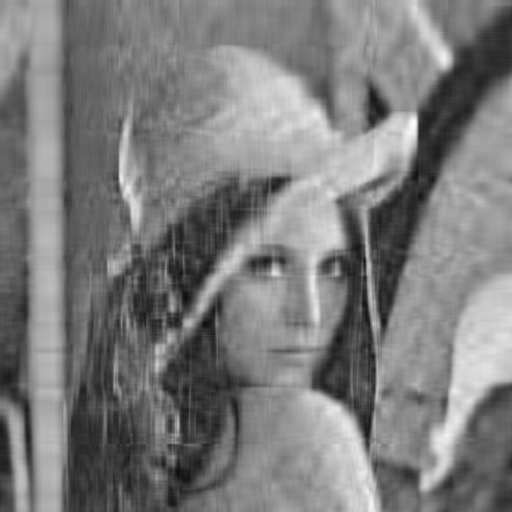
\includegraphics[width=\textwidth]{../resultados/reconstrucciones/ak_3_20.png}
    \caption{$k=20$}
\end{subfigure}
\hfill
\begin{subfigure}[b]{0.18\textwidth}
    \centering
    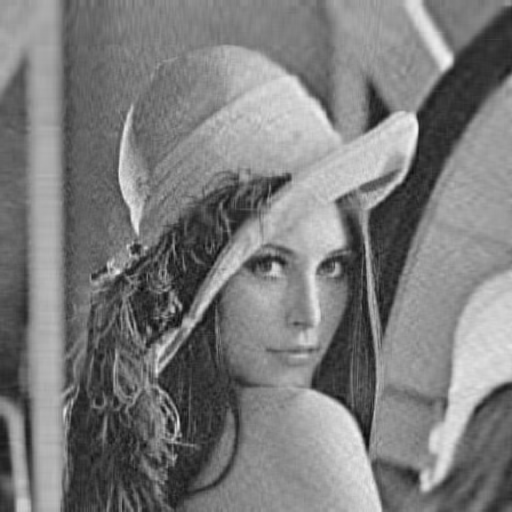
\includegraphics[width=\textwidth]{../resultados/reconstrucciones/ak_3_50.png}
    \caption{$k=50$}
\end{subfigure}
\hfill
\begin{subfigure}[b]{0.18\textwidth}
    \centering
    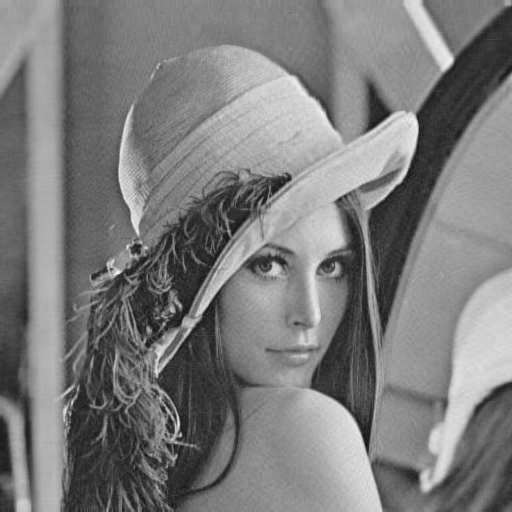
\includegraphics[width=\textwidth]{../resultados/reconstrucciones/ak_3_100.png}
    \caption{$k=100$}
\end{subfigure}
\hfill
\begin{subfigure}[b]{0.18\textwidth}
    \centering
    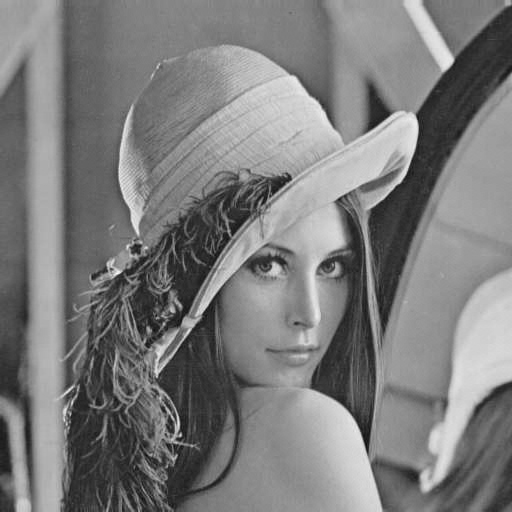
\includegraphics[width=\textwidth]{../resultados/reconstrucciones/ak_3_200.png}
    \caption{$k=200$}
\end{subfigure}
\caption{Reconstrucciones de Lena (gris) para $k \in \{5, 20, 50, 100, 200\}$. Con $k=50$ la imagen ya es visualmente indistinguible del original.}
\label{fig:lena-gris-reconstrucciones}
\end{figure}

\subsubsection{Lena RGB (ID 6)}
\begin{figure}[H]
\centering
\begin{subfigure}[b]{0.18\textwidth}
    \centering
    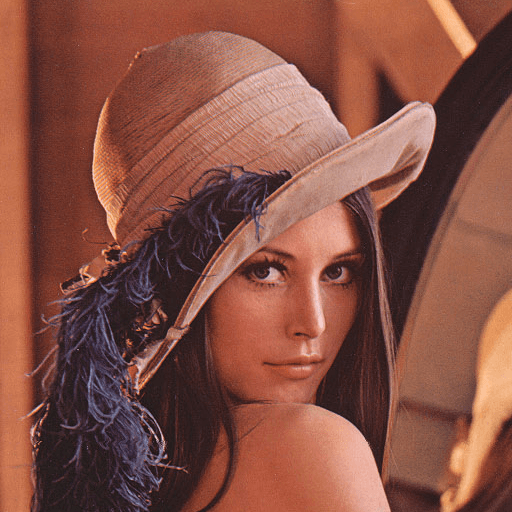
\includegraphics[width=\textwidth]{../assets/rgb/lena_rgb_6.png}
    \caption{Original}
\end{subfigure}
\hfill
\begin{subfigure}[b]{0.18\textwidth}
    \centering
    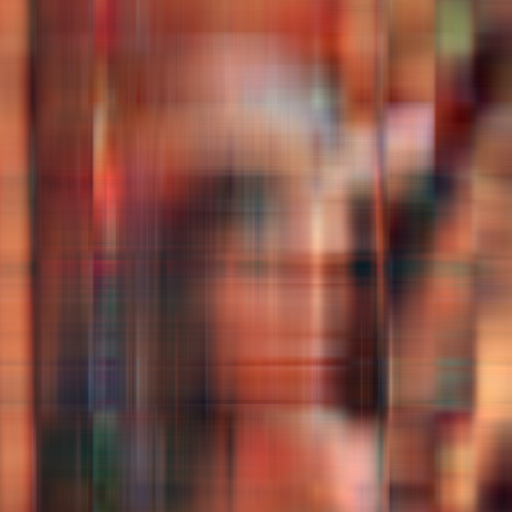
\includegraphics[width=\textwidth]{../resultados/reconstrucciones/ak_6_5.png}
    \caption{$k=5$}
\end{subfigure}
\hfill
\begin{subfigure}[b]{0.18\textwidth}
    \centering
    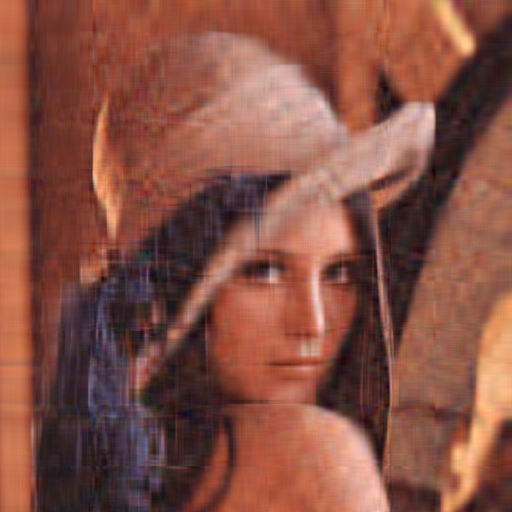
\includegraphics[width=\textwidth]{../resultados/reconstrucciones/ak_6_20.png}
    \caption{$k=20$}
\end{subfigure}
\hfill
\begin{subfigure}[b]{0.18\textwidth}
    \centering
    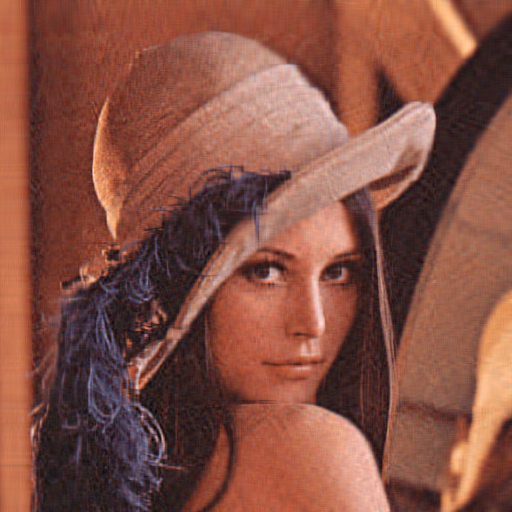
\includegraphics[width=\textwidth]{../resultados/reconstrucciones/ak_6_50.png}
    \caption{$k=50$}
\end{subfigure}
\hfill
\begin{subfigure}[b]{0.18\textwidth}
    \centering
    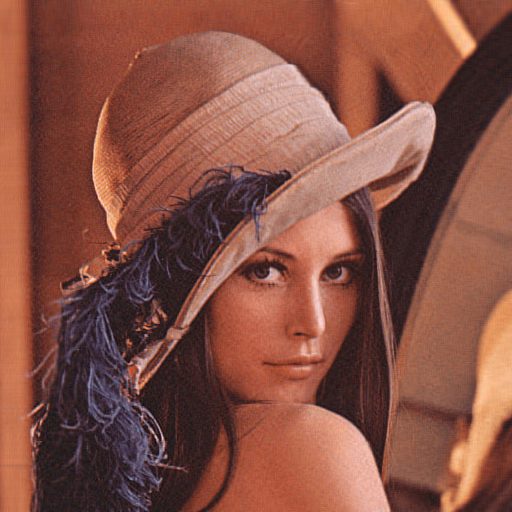
\includegraphics[width=\textwidth]{../resultados/reconstrucciones/ak_6_100.png}
    \caption{$k=100$}
\end{subfigure}
\hfill
\begin{subfigure}[b]{0.18\textwidth}
    \centering
    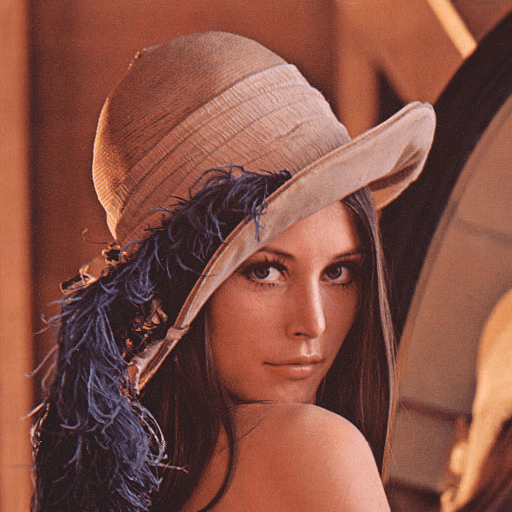
\includegraphics[width=\textwidth]{../resultados/reconstrucciones/ak_6_200.png}
    \caption{$k=200$}
\end{subfigure}
\caption{Reconstrucciones de Lena (RGB) para $k \in \{5, 20, 50, 100, 200\}$. Con $k=100$ la imagen ya es visualmente indistinguible del original.}
\label{fig:lena-rgb-reconstrucciones}
\end{figure}

\subsubsection{Mandril RGB (ID 7)}

\begin{figure}[H]
\centering
\begin{subfigure}[b]{0.18\textwidth}
    \centering
    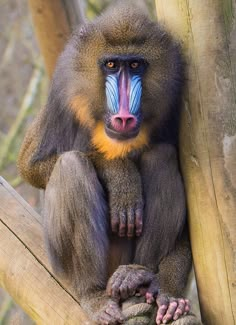
\includegraphics[width=\textwidth]{../assets/rgb/mandril_rgb_7.png}
    \caption{Original}
\end{subfigure}
\hfill
\begin{subfigure}[b]{0.18\textwidth}
    \centering
    
\includegraphics[width=\textwidth]{../resultados/reconstrucciones/ak_7_5.png}
    \caption{$k=5$}
\end{subfigure}
\hfill
\begin{subfigure}[b]{0.18\textwidth}
    \centering
    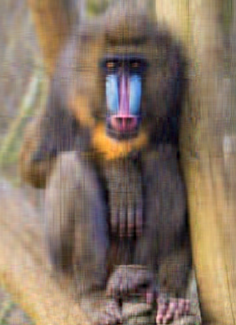
\includegraphics[width=\textwidth]{../resultados/reconstrucciones/ak_7_20.png}
    \caption{$k=20$}
\end{subfigure}
\hfill
\begin{subfigure}[b]{0.18\textwidth}
    \centering
    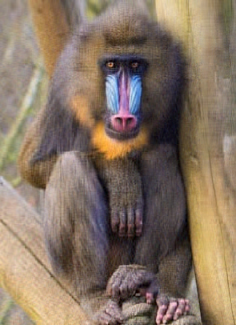
\includegraphics[width=\textwidth]{../resultados/reconstrucciones/ak_7_50.png}
    \caption{$k=50$}
\end{subfigure}
\hfill
\begin{subfigure}[b]{0.18\textwidth}
    \centering
    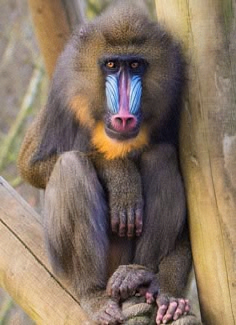
\includegraphics[width=\textwidth]{../resultados/reconstrucciones/ak_7_100.png}
    \caption{$k=100$}
\end{subfigure}
\hfill
\begin{subfigure}[b]{0.18\textwidth}
    \centering
    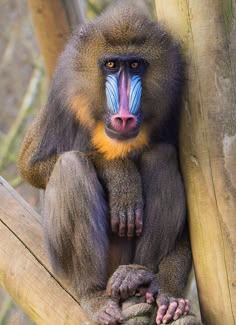
\includegraphics[width=\textwidth]{../resultados/reconstrucciones/ak_7_200.png}
    \caption{$k=200$}
\end{subfigure}
\caption{Reconstrucciones de Mandril (RGB) para $k \in \{5, 20, 50, 100, 200\}$. Con $k=50$ la imagen ya es visualmente indistinguible del original.}
\label{fig:mandril-rgb-reconstrucciones}
\end{figure}

\subsubsection{Pimiento RGB (ID 8)}

\begin{figure}[H]
\centering
\begin{subfigure}[b]{0.18\textwidth}
    \centering
    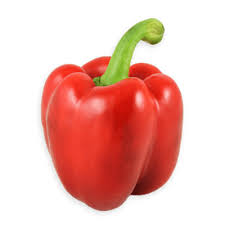
\includegraphics[width=\textwidth]{../assets/rgb/pimiento_rgb_8.png}
    \caption{Original}
\end{subfigure}
\hfill
\begin{subfigure}[b]{0.18\textwidth}
    \centering
    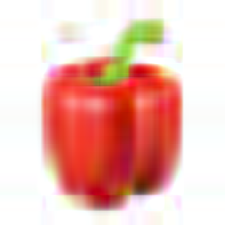
\includegraphics[width=\textwidth]{../resultados/reconstrucciones/ak_8_5.png}
    \caption{$k=5$}
\end{subfigure}
\hfill
\begin{subfigure}[b]{0.18\textwidth}
    \centering
    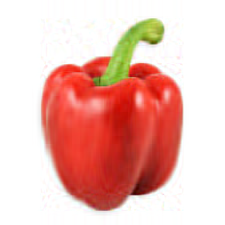
\includegraphics[width=\textwidth]{../resultados/reconstrucciones/ak_8_20.png}
    \caption{$k=20$}
\end{subfigure}
\hfill
\begin{subfigure}[b]{0.18\textwidth}
    \centering
    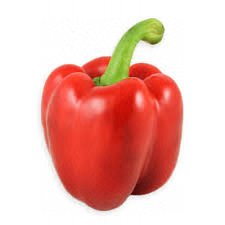
\includegraphics[width=\textwidth]{../resultados/reconstrucciones/ak_8_50.png}
    \caption{$k=50$}
\end{subfigure}
\hfill
\begin{subfigure}[b]{0.18\textwidth}
    \centering
    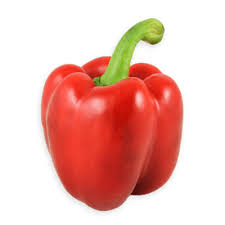
\includegraphics[width=\textwidth]{../resultados/reconstrucciones/ak_8_100.png}
    \caption{$k=100$}
\end{subfigure}
\hfill
\begin{subfigure}[b]{0.18\textwidth}
    \centering
    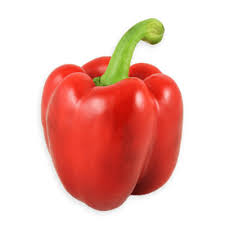
\includegraphics[width=\textwidth]{../resultados/reconstrucciones/ak_8_200.png}
    \caption{$k=200$}
\end{subfigure}
\caption{Reconstrucciones de Pimiento (RGB) para $k \in \{5, 20, 50, 100, 200\}$. Con $k=20$ la imagen ya es visualmente indistinguible del original.}
\label{fig:pimiento-rgb-reconstrucciones}
\end{figure}

% ---------- 5. ANALISIS COMPARATIVO ----------
\section{An\'{a}lisis Comparativo}\label{sec:analisis}

\subsection{Compresibilidad por Tipo de Imagen}

Los resultados obtenidos revelan tres patrones distintivos:

\begin{enumerate}
    \item \textbf{Alta compresibilidad (pimiento, mandril rgb):} Im\'{a}genes con regiones de color homog\'{e}neo y bordes suaves. Con $k=20$ se captura $>$99.5\% de la energ\'{i}a y el error relativo es $<$2\%. La tasa de compresi\'{o}n supera $5\times$ sin p\'{e}rdida perceptible.

    \item \textbf{Compresibilidad media (Lena, edificio):} Texturas moderadas. Requieren $k=50$ para alcanzar $>$99.5\% de energ\'{i}a. La tasa de compresi\'{o}n a ese nivel es $\sim 5\times$.

    \item \textbf{Baja compresibilidad (geometr\'{i}a):} Figuras sint\'{e}ticas con bordes n\'{i}tidos y alta variabilidad espectral. Incluso con $k=100$ solo se alcanza 90.2\% de energ\'{i}a, requiriendo $k=200$ (casi rango completo) para obtener calidad aceptable.
\end{enumerate}

\subsection{Escala de Grises vs. RGB}

Las im\'{a}genes RGB procesadas canal por canal exhiben comportamientos cuantitativos similares a sus contrapartes en escala de grises (Tabla~\ref{tab:resumen}, IDs 3 vs.\ 6, 4 vs.\ 7). Esto confirma que la correlaci\'{o}n espacial es la variable dominante, no el modo de color. La penalizaci\'{o}n de compresi\'{o}n en RGB es exactamente $3\times$ en datos almacenados, pero las tasas reportadas en la Tabla~\ref{tab:resumen} ya consideran esta multiplicaci\'{o}n.

\subsection{Verificaci\'{o}n del Teorema de Eckart-Young-Mirsky}

El test unitario de reconstrucci\'{o}n exacta ($k=r$) arroj\'{o} un error relativo de $4.75 \times 10^{-15}$, confirmando que \texttt{BDCSVD} preserva la ortogonalidad y la factorizaci\'{o}n exacta dentro de la precisi\'{o}n de m\'{a}quina. Adem\'{a}s, el error relativo decrece mon\'{o}tonamente con $k$ en todas las im\'{a}genes, comportamiento consistente con la optimalidad del Teorema~\ref{thm:eym}.

% ---------- 6. CONCLUSIONES ----------
\section{Conclusiones}\label{sec:conclusiones}

\begin{enumerate}
    \item Se implement\'{o} exitosamente un pipeline completo de compresi\'{o}n SVD en C++17, desde la carga de im\'{a}genes hasta la exportaci\'{o}n de m\'{e}tricas y gr\'{a}ficos, con arquitectura modular y sin dependencias externas pesadas (Eigen es header-only).

    \item El algoritmo \texttt{BDCSVD} de Eigen demostr\'{o} ser num\'{e}ricamente estable y eficiente para matrices de imagen, con errores de reconstrucci\'{o}n exacta del orden de la precisi\'{o}n de m\'{a}quina ($\sim 10^{-15}$).

    \item Las im\'{a}genes naturales con texturas suaves (pimiento, Lena, mandril) son altamente compresibles mediante SVD, alcanzando tasas $>$5$\times$ con p\'{e}rdida de energ\'{i}a $<$1\%. Las im\'{a}genes sint\'{e}ticas con alta frecuencia espacial (geometr\'{i}a) requieren rangos cercanos al completo.

    \item El procesamiento por canales independientes en RGB es v\'{a}lido y produce m\'{e}tricas comparables a las im\'{a}genes en escala de grises, con la penalizaci\'{o}n esperada de $3\times$ en volumen de datos.
\end{enumerate}

% ---------- REFERENCIAS ----------
\begin{thebibliography}{9}
\bibitem{eigen} Eigen Documentation. \textit{SVD Module.} \url{https://eigen.tuxfamily.org/dox/group__SVD__Module.html}
\bibitem{golub} Golub, G. H., \& Van Loan, C. F. (2013). \textit{Matrix Computations} (4th ed.). Johns Hopkins University Press.
\bibitem{demofox} DemoFox Blog. (2022). \textit{Calculating SVD and PCA in C++.} \url{https://blog.demofox.org/2022/07/12/calculating-svd-and-pca-in-c/}
\bibitem{compton} Compton, A. (2020). \textit{Singular Value Decomposition: Applications to Image Processing.} Lagrange University Undergraduate Research.
\bibitem{stb} stb Libraries. \url{https://github.com/nothings/stb}
\end{thebibliography}

\end{document}
    